\chapter{Evaluation}
\label{chp:evaluation}

Nachdem im letzten Kapitel die unterschiedlichen Klauselmengen bewertet wurden, wird die Klauselmenge aus Abschnitt \ref{sec:test_beste}
in diesem Kapitel für die Evaluation herangezogen. Bisher wurden Klauseln mit Hilfe von acht Threads in CryptoMiniSat ermittelt und bewertet.
Da mit dieser Konfiguration auch Werte geraten werden, hat das zu unterschiedlichen Ergebnissen und Laufzeiten geführt. Um dieses Verhalten
zu vermeiden, wird die Evaluation mit nur einem Thread durchgeführt, dessen Standardkonfiguration ein deterministisches Verhalten bewirkt
und somit in annähernd gleicher Zeit immer zum selben Ergebnis führt.

Während die Implementierung dieser Arbeit im folgenden Abschnitt zunächst mit den Implementierungen von \acr{cbmc} und Martin Maurer verglichen wird,
erfolgt im Anschluss eine Bewertung, ob praktische relevante Angriffe auf \glos{sha256} und Bitcoin möglich sind.

\section{Vergleich}

\TODO{erledigen}

\subsection{CBMC}

\subsection{capiman}
\section{Bedeutung für SHA-256}

Die Versuche aus Kapitel \ref{chp:bewertung} und Abschnitt \ref{sec:vergleich} zeigen, dass sich innerhalb eines Tages
ein Urbild für einen \glos{hash} berechnen lässt, der je nach Implementierung mit 18 bis 20 festgelegten Bits beginnt. Das ist jedoch
kein Vergleich zum Ergebnis, das sich durch reines Probieren erzielen lässt. In der Testumgebung können 720.000 \glospl{hash} pro Sekunde
berechnet werden. Damit ist es möglich innerhalb eines Tages ein Urbild für einen \glos{hash} mit bis zu 35 festgelegten Bits zu finden.

\subsection{Initialwertberechnung}
Abschnitt \ref{sec:initialwertberechnung} beschreibt den Sinn einer Initialwertberechnung. Diese wird im folgenden separat
betrachtet, da die Erweiterung der Eingabe (siehe Abschnitt \ref{sec:sha256:erweiterung}) vollständig berechnet werden kann
und somit durch einen SAT-Solver nicht mehr betrachtet werden braucht. Das Problem reduziert sich damit auf die Berechnung
der 64 Runden. Abbildung \ref{fig:eval_initial} zeigt das Ergebnis dieses Versuchs im Vergleich zur Urbildberechnung.
\begin{figure}[!h]
  \centering
  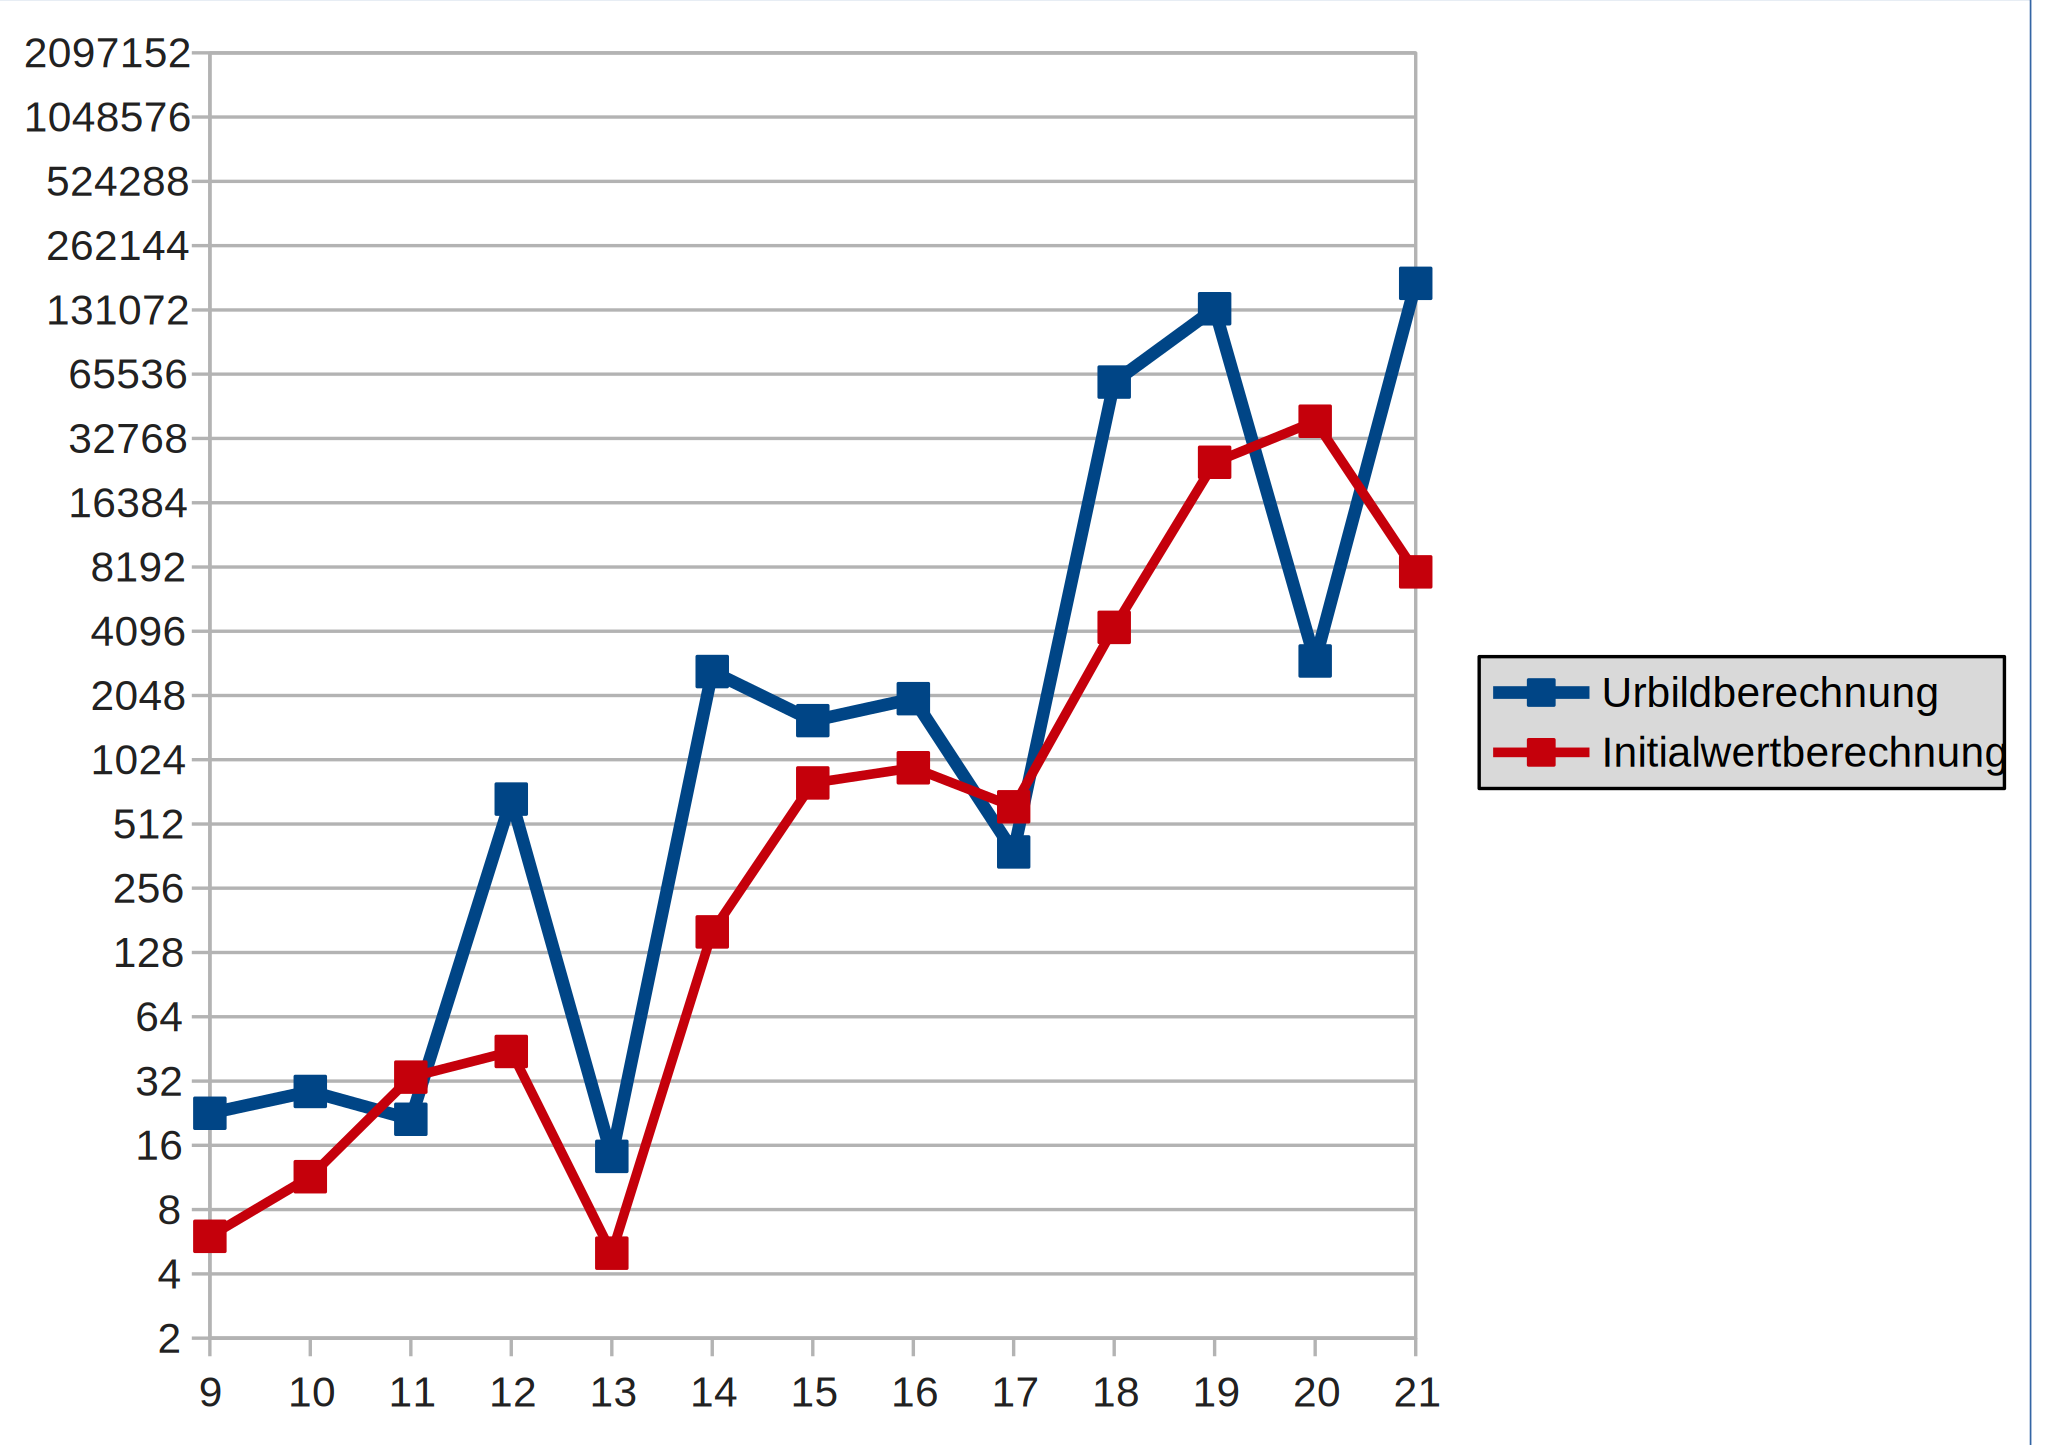
\includegraphics[scale=0.55]{images/eval_initial}
  \caption{Evaluation - Initialwertberechnung}
  \label{fig:eval_initial}
\end{figure}

Während die Urbildberechnung insgesamt 105 Stunden benötigt hat, wurde die Initialwertberechnung in 22 Stunden
abgeschlossen. Mit drei Ausnahmen war die Initialwertberechnung in allen Fällen schneller als die Urbildberechnung.

\subsection{Kollisionsberechnung}
Abschließend wird die in Abschnitt \ref{sec:kollisionsberechnung} beschriebene Kollisionsberechnung durchgeführt.
Abbildung \ref{fig:eval_kollision} zeigt das Ergebnis im Vergleich zur Urbildberechnung. \clearpage
\begin{figure}[!h]
  \centering
  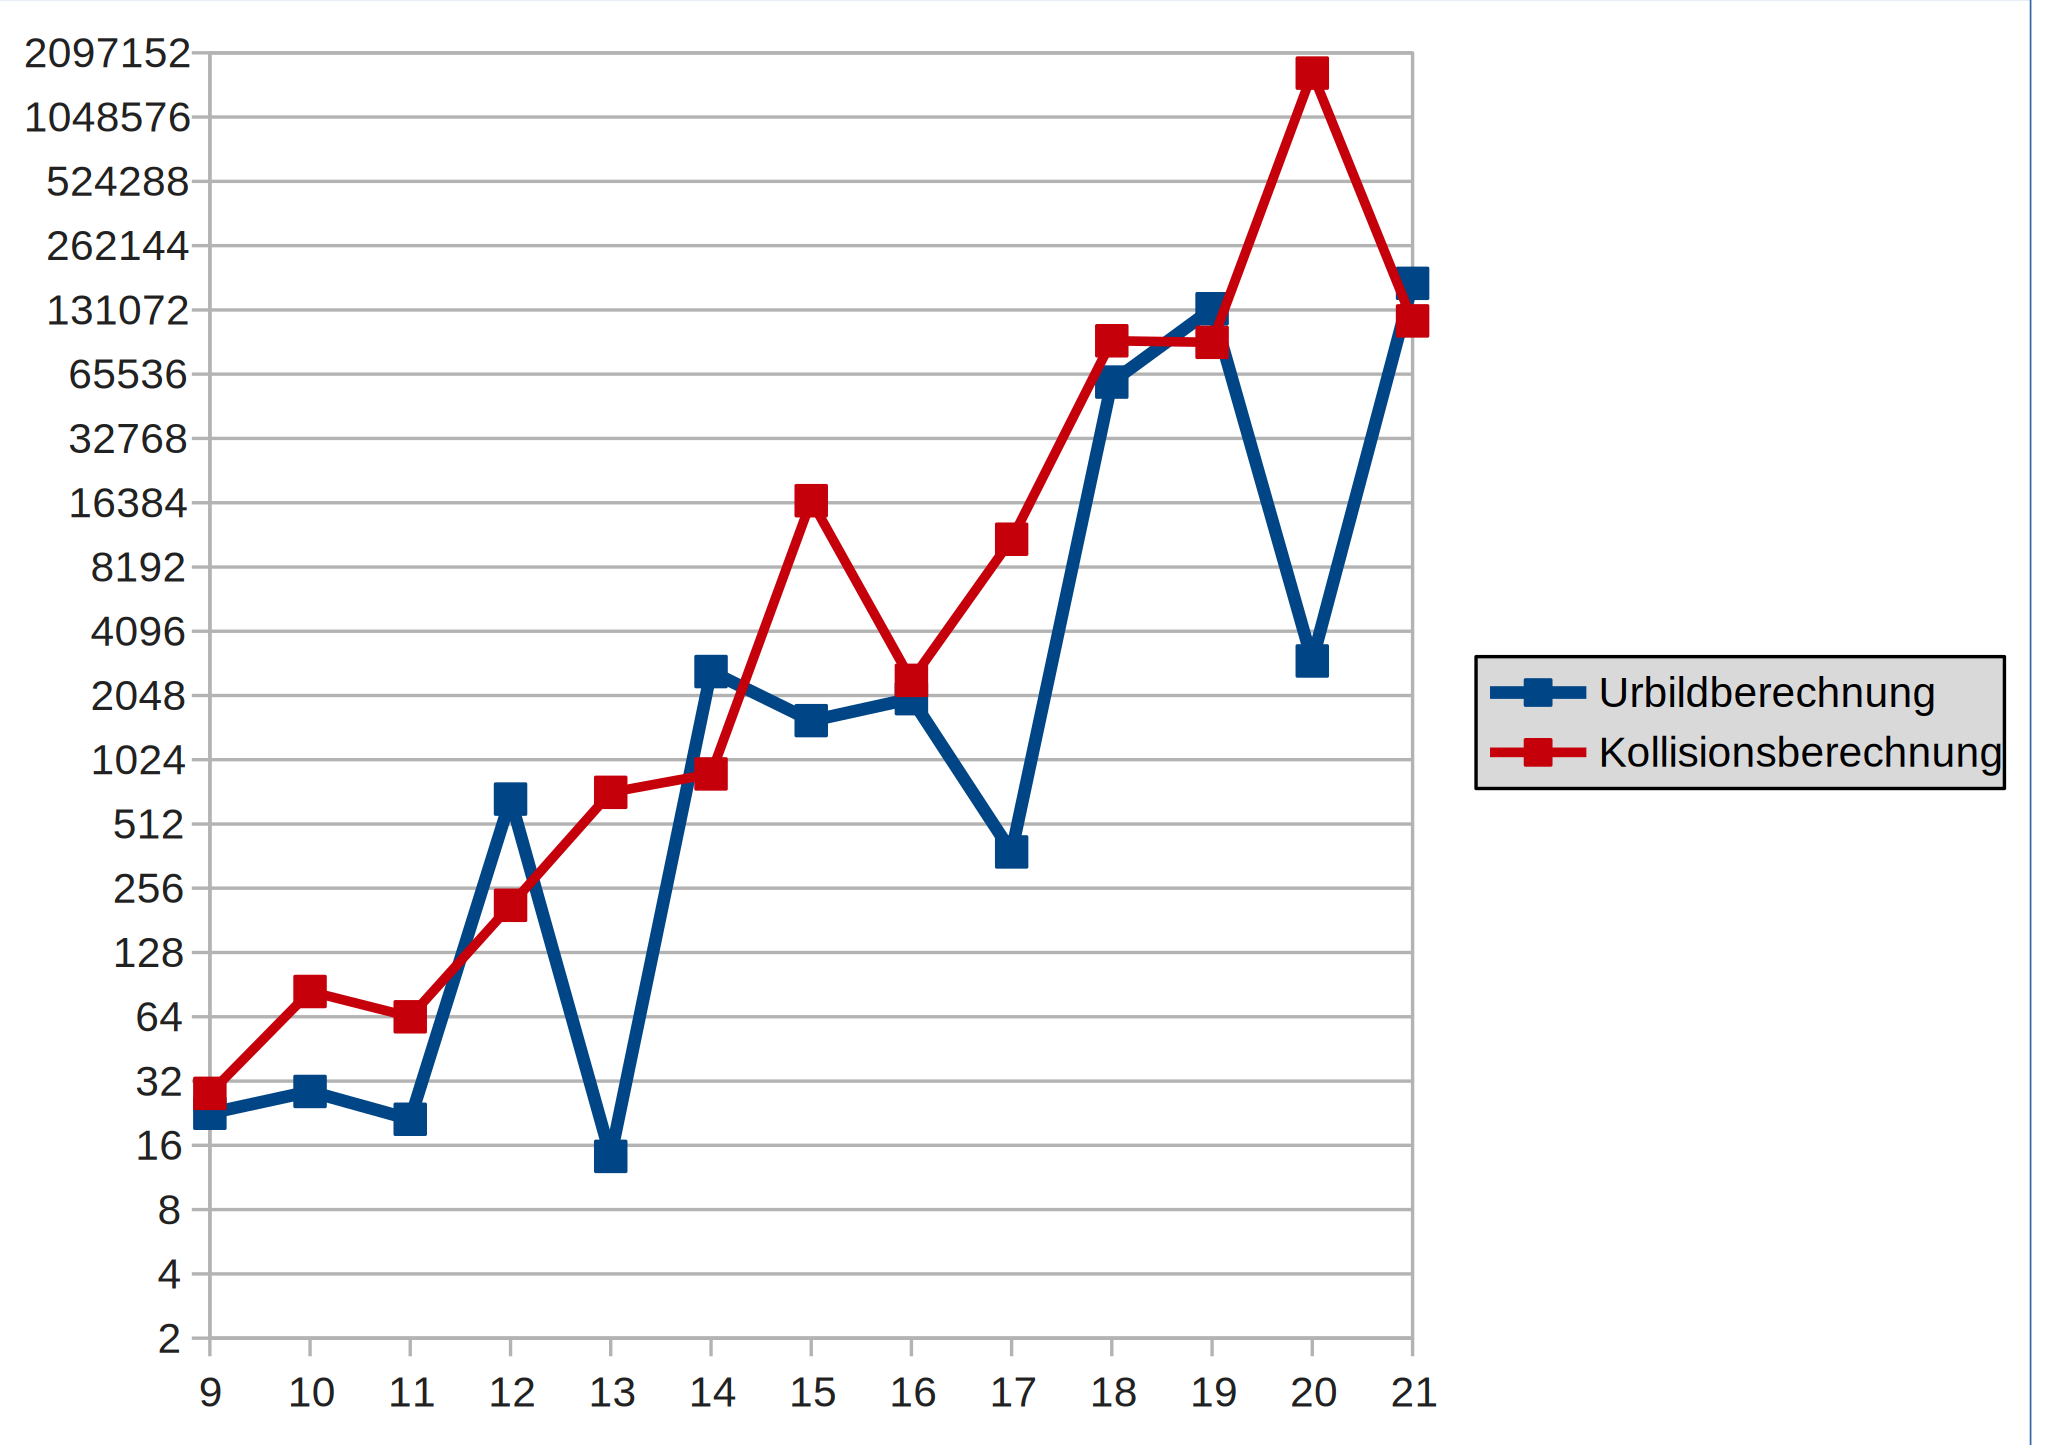
\includegraphics[scale=0.55]{images/eval_kollision}
  \caption{Evaluation - Kollisionsberechnung}
  \label{fig:eval_kollision}
\end{figure}

Es zeigt sich, dass die freie Wahl eines \glos{hash} für CryptoMiniSat keinen Vorteil darstellt. In den meisten Fällen
dauert eine Kollisionsberechnung länger als eine Urbildberechnung.
\section{Bedeutung für das Bitcoin-Mining}

Jonathan Heusser führt in seinem Artikel \cite{jona:1} zwei Versuche mit unterschiedlichen SAT-Solvern durch.
Diese ließen sich für einen direkten Vergleich leider nicht reproduzieren, da die vom ihm genutzte konjunktive
Normalform unterschiedlich zu der ist, die sich mit \acr{cbmc} aus seinem C-Programmcode erstellen lässt.
Außerdem gibt er in seinen Versuchen eine feste Anzahl führender Nullen für den Hash vor und variiert die
Anzahl der Stellen der Nonce die noch berechnet werden müssen um die Schwierigkeit zu verändern. Das eignet
sich zwar für den Vergleich unterschiedlicher SAT-Solver, ermöglicht jedoch keine direkte Aussage dazu, ob
sich dieses Vorgehen dafür eignet aktuelle Bitcoin-Blöcke zu lösen.

In der Praxis ist die Nonce vollständig unbekannt und die Schwierigkeit wird dadurch angepasst, dass die Anzahl
der geforderten führenden Nullen sich ändert. Ziel von Bitcoin ist es, die Schwierigkeit immer so anzupassen, dass im Mittel
alle zehn Minuten ein Block gelöst wird. Damit stellt sich die Frage, bei wie vielen führenden Nullen der SAT-Solver
innerhalb von 10 Minuten zu einer Lösung kommt. Tabelle \ref{fig:bitcoinzeros} zeigt die Ergebnisse der mit CryptoMiniSat
durchgeführten Versuche.

\begin{table}[!h]
  \centering
  \begin{tabular}{rr|rr}
    Geforderte Nullen & Dauer in Minuten & Erhaltene Nullen \\
    \hline
     9 &  0:43 &  9 \\
    10 &  1:55 & 10 \\
    11 &  8:32 & 11 \\
    12 &  5:29 & 14 \\
    13 & 10:39 & 16
  \end{tabular}
  \caption{Erworbene Klauseln in der Kompressionsfunktion nach Bereinigung}
  \label{fig:bitcoinzeros}
\end{table}

Für jede Anzahl der geforderten Nullen wurden jeweils fünf Versuche durchgeführt, die durch eine Zeile in Tabelle \ref{fig:bitcoinzeros}
repräsentiert werden. Es hat sich gezeigt, dass CryptoMiniSat innerhalb jeder Versuchsreihe jeweils die selbe Nonce ermittelt hat
und die Dauer nur wenig variierte. Die angegebene Dauer ist der arithmetische Mittelwert. Die letzte Spalte enthält die Anzahl der
führenden Nullen die tatsächlich erreicht wurden. Da ein SAT-Solver die nicht festgelegten Stellen frei belegen kann, ist es möglich,
dass das Ergebnis mehr führende Nullen hat als gefordert. Dies ist jedoch zufällig und nur zur Vollständigkeit mit aufgeführt.
In annähernd zehn Minuten ist es somit möglich eine Nonce für einen Hash mit bis zu 13 führenden Nullen zu ermitteln.

Da die aktuellen Blöcke einen Hash mit mindestens 68 führenden Nullen erfordern, zeigt dieser Versuch, dass SAT-Solving sich
derzeit nicht für den Einsatz in Bitcoin-Minern eignet. Betrachtet werden muss auch, dass in der Testumgebung 720.000 Hashes pro Sekunde
berechnet werden können. Damit kann alleine durch Probieren in zehn Minuten eine gültige Nonce für einen Hash mit 27 führenden
Nullen ermittelt werden.